\chapter{Krylov Methods and GMRES}
\label{chpt:GMRES}



In Chapter~\ref{chpt:FDM}, every problem ended with a linear system of the form
$A\mathbf{u} = \mathbf{f}$, which we solved with a single call to
\texttt{A\textbackslash f} or \texttt{spsolve}. In one dimension this is
perfectly reasonable: the matrix is tridiagonal and a direct solver handles it
in $\mathcal{O}(N)$ work. In three dimensions, a modest grid
of $N = 128$ points per direction carries $N^3 \approx 2\times10^6$
unknowns making linear solvers unreasonable. This chapter introduces a different
strategy: rather than solve the system exactly, we build an increasingly good
approximation to the solution from a small set of carefully chosen vectors.
The method we focus on, the \emph{Generalized Minimal RESidual} method
(GMRES), has three features:
\begin{enumerate}
  \item it never needs the matrix itself, only a way to \emph{apply} the matrix
        to a vector;
  \item it is iterative, so it needs an initial guess;
  \item it is approximate, so it needs a stopping tolerance.
\end{enumerate}
\index{GMRES}\index{iterative methods}

\section{A Model Problem: Poisson's Equation in Three Dimensions}
\label{sec:gmres-model}

Consider Poisson's equation on the cube $\Omega = [0,2\pi]^3$ with homogeneous
Dirichlet boundary conditions,
\begin{equation}
  \nabla^2 u = f, \qquad
  u \Big|_{\partial\Omega} = 0,
  \label{eq:gmres-poisson}
\end{equation}
where
$\nabla^2 = \frac{\partial^2}{\partial x^2} + \frac{\partial^2}{\partial y^2}
+ \frac{\partial^2}{\partial z^2}$.
To check our numerical solutions we choose the manufactured solution
\begin{equation}
  u(x,y,z) = e^{\sin x \,\sin y\, \sin z} - 1,
  \label{eq:gmres-exact}
\end{equation}
which vanishes on every face of the cube, and compute $f = \nabla^2 u$ by hand.
\index{manufactured solution}

\begin{exercise}
Verify that \eqref{eq:gmres-exact} satisfies the boundary condition in
\eqref{eq:gmres-poisson} and compute $f = \nabla^2 u$.
\end{exercise}

\subsection{Discretization}

We use the Type~I grid of Section~\ref{sec:typeI} in each direction and
treat the Dirichlet values as known, removing them from the system exactly as
in \eqref{rhsDirTop}. Because the boundary values are zero, no correction to
the right-hand side is needed. To keep the code compact we now let $N$ denote
the number of \emph{interior} points in each direction, so
\begin{equation}
  x_i = i\,\Delta x, \qquad i = 1,\dots,N, \qquad \Delta x = \frac{2\pi}{N+1},
\end{equation}
and likewise for $y_j$ and $z_k$. We write $u_{i,j,k} \approx u(x_i,y_j,z_k)$.

Applying the second-order central difference \eqref{eq:fdSecond} in each
direction gives the \emph{seven-point Laplacian}. We extend our compass
notation to three dimensions: about the point $P = (i,j,k)$ the neighbors are
east/west ($E,W$) in $x$, north/south ($N,S$) in $y$, and top/bottom ($T,B$)
in $z$. Then
\begin{equation}
  \nabla^2 u \big|_P \approx
  \frac{u_E + u_W + u_N + u_S + u_T + u_B - 6\,u_P}{\Delta x^2}.
  \label{eq:gmres-7pt}
\end{equation}
The notation $u_E$ denotes $u$ as evaluated at $u(i + 1, j, k)$ and $u_T = u(i, j, k + 1)$.
\index{seven-point Laplacian}

\begin{figure}[htbp]
  \centering
  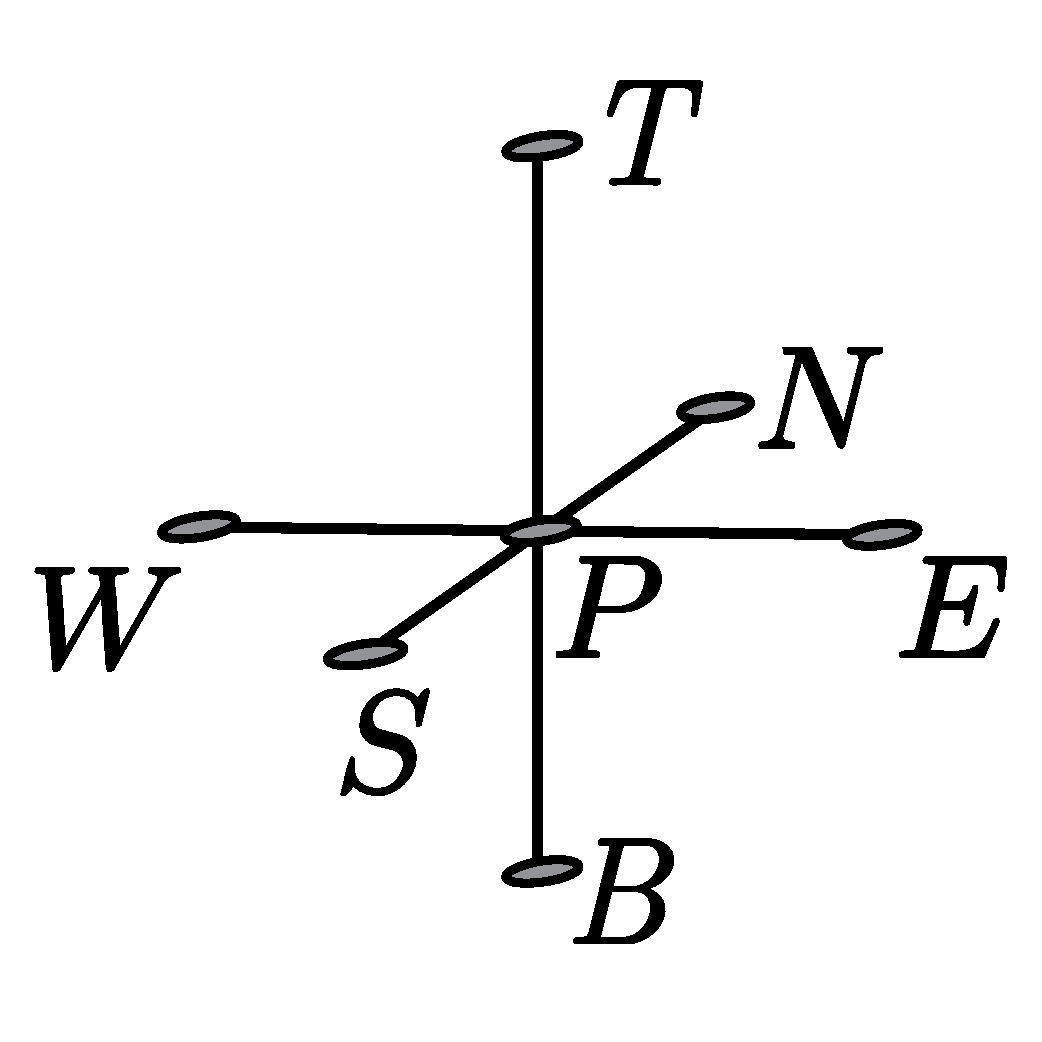
\includegraphics[width=0.6\linewidth]{GMRES/Images/GMRES.pdf}
  \caption{The seven-point stencil for the three-dimensional Laplacian. The
  center point $P$ should be highlighted, with its six neighbors $E, W$ (along
  $x$), $N, S$ (along $y$), and $T, B$ (along $z$) labelled in the compass
  notation and connected to $P$.}
  \label{fig:gmres-stencil}
\end{figure}

\begin{exercise}
What is the local truncation error of \eqref{eq:gmres-7pt}? Use the
one-dimensional result of Section~\ref{sec:secondderiv} rather than redoing a
three-dimensional Taylor expansion. What order of convergence should we expect
for the solution $u$?
\end{exercise}

\subsection{Assembling the matrix}

Stacking the $N^3$ unknowns row-wise into a single vector $\mathbf{u}$ turns
\eqref{eq:gmres-7pt} into a linear system $L\mathbf{u} = \mathbf{f}$. The
matrix $L$ can be built from the one-dimensional matrix
$D_2 \in \mathbb{R}^{N\times N}$ using Kronecker products, as we did for 2D, such that
\begin{equation}
  L = I \otimes I \otimes D_2 \;+\; I \otimes D_2 \otimes I
      \;+\; D_2 \otimes I \otimes I ,
  \label{eq:gmres-kron}
\end{equation}
where $I$ is the $N\times N$ identity. Recall that for
$A\in\mathbb{R}^{m\times n}$ and $B$ of any size,
\[
  A \otimes B =
  \begin{bmatrix}
    a_{11}B & \cdots & a_{1n}B \\
    \vdots  & \ddots & \vdots \\
    a_{m1}B & \cdots & a_{mn}B
  \end{bmatrix}.
\]
\index{Kronecker product}


The matrix $L$ is sparse, but its bandwidth is $N^2$. A direct solver such as
Gaussian elimination fills in much of that band as it factors $L$, so both
the memory and the work grow far faster than the $\mathcal{O}(N^3)$ nonzeros
of $L$ itself. 

\begin{remark}
For large problems in two and especially three dimensions, \emph{how} we
solve $L\mathbf{u} = \mathbf{f}$ matters as much as how we discretized the
PDE. A good discretization paired with a solver that cannot finish is not
useful.
\end{remark}

\section{Krylov Subspaces}
\label{sec:krylov}

Let $A\in\mathbb{R}^{n\times n}$ be nonsingular and consider $A\mathbf{x} =
\mathbf{b}$. The goal of Krylov methods is to build a vector space $\mathcal{K}_k$ using $\mathbf{b}$ and repeated
multiplication by $A$ such that $\mathbf{x} \in \mathcal{K}_k$.

\begin{definition}[Krylov subspace]
The $k$-th Krylov subspace generated by $A$ and $\mathbf{b}$ is
\[
  \mathcal{K}_k(A,\mathbf{b}) =
  \operatorname{span}\left\{\mathbf{b},\, A\mathbf{b},\, A^2\mathbf{b},\,
  \dots,\, A^{k-1}\mathbf{b}\right\}.
\]
\end{definition}
\index{Krylov subspace}

Every vector in $\mathcal{K}_k(A,\mathbf{b})$ has the form
$p(A)\,\mathbf{b}$ for some polynomial $p$ of degree at most $k-1$. $A^{-1}$ can be written in the form $p(A)$ for some polynomial $p$ of degree at most $n-1$, as $A$ satisfies its own characteristic polynomial following from the Cayley--Hamilton theorem. Therefore
$\mathbf{x} = A^{-1}\mathbf{b} \in \mathcal{K}_n(A,\mathbf{b})$. The hope of
every Krylov method is that $\mathcal{K}_k$ contains a good approximation of $A^{-1}$ for $k \ll n$.
\index{Cayley--Hamilton theorem}


\subsection{Only the action of $A$ is needed}
\label{sec:matfree-idea}

Consider the basis $\{\mathbf{b}, A\mathbf{b}, A^2\mathbf{b},\dots\}$.
To build it we need exactly two things:
\begin{enumerate}
  \item the vector $\mathbf{b}$, and
  \item a procedure that takes a vector $\mathbf{v}$ and returns $A\mathbf{v}$.
\end{enumerate}
We never need to look at an individual entry $a_{ij}$ or store $A$. Any function that computes $\mathbf{v}\mapsto A\mathbf{v}$ will do.
Operators that exploit this are called \emph{matrix-free} methods.
\index{matrix-free methods} Utilizing these matrix-free methods allow us to recover  $L\mathbf{u}$ without ever building or operating with $L$. Compare this with getting the Kronecker
structure of \eqref{eq:gmres-kron} right or with assembling a matrix for a
more complicated operator. The
function \texttt{Apply\_Lap} in Section~\ref{sec:gmres-code} is a
matrix-free implementation of $L$.

\begin{exercise}
In \texttt{Apply\_Lap}, the neighbor values \texttt{u\_E}, \texttt{u\_W},
$\dots$ are initialized to zero and only overwritten when the neighbor is
inside the grid. Explain why this implements the boundary condition in
\eqref{eq:gmres-poisson}. How would you modify the function if the Dirichlet
value on the face $x = 0$ were a nonzero constant $\alpha$? (Hint: think about
what is linear and what is not, and look back at \eqref{rhsDirTop}.) How would
you implement a Neumann condition on that face using the ghost points of
Section~\ref{sec:bc-neumann}?
\end{exercise}

\subsection{Building a good basis: the Arnoldi process}
\label{sec:arnoldi}

In floating point arithmetic the vectors $A^{k}\mathbf{b}$ are a poor basis as they share common eigenvectors. Instead we
build an \emph{orthonormal} basis $\mathbf{q}_1,\dots,\mathbf{q}_k$ for the
same space one vector at a time by multiplying the newest basis vector by $A$, then
orthogonalizing the result against all previous vectors with Gram--Schmidt. This
is called the Arnoldi process and laid out in Algorithm~\ref{alg:arnoldi}.
\index{Arnoldi process}

\begin{algorithm}[htbp]
\caption{Arnoldi process (modified Gram--Schmidt)}
\label{alg:arnoldi}
\begin{algorithmic}[1]
\State $\mathbf{q}_1 \gets \mathbf{r}_0 / \norm{\mathbf{r}_0}_2$
\For{$j = 1, 2, \dots, k$}
  \State $\mathbf{w} \gets A\,\mathbf{q}_j$ \Comment{the only use of $A$}
  \For{$i = 1, \dots, j$}
    \State $h_{ij} \gets \mathbf{q}_i^T \mathbf{w}$
    \State $\mathbf{w} \gets \mathbf{w} - h_{ij}\,\mathbf{q}_i$
  \EndFor
  \State $h_{j+1,j} \gets \norm{\mathbf{w}}_2$
  \State $\mathbf{q}_{j+1} \gets \mathbf{w} / h_{j+1,j}$
\EndFor
\end{algorithmic}
\end{algorithm}

Collecting the basis vectors into $Q_k = [\mathbf{q}_1 \cdots \mathbf{q}_k]$
and the coefficients $h_{ij}$ into the $(k+1)\times k$ upper Hessenberg matrix
$\widetilde{H}_k$, the Arnoldi process produces the relation
\begin{equation}
  A\,Q_k = Q_{k+1}\,\widetilde{H}_k .
  \label{eq:arnoldi}
\end{equation}


\section{The GMRES Algorithm}
\label{sec:gmres}

Given an initial guess $\mathbf{x}_0$ with residual
$\mathbf{r}_0 = \mathbf{b} - A\mathbf{x}_0$, GMRES chooses the $k$-th iterate
as the vector in the shifted Krylov space that makes the residual as small as
possible, such that
\begin{equation}
  \mathbf{x}_k = \operatorname*{arg\,min}_{\mathbf{x}\,\in\,\mathbf{x}_0 +
  \mathcal{K}_k(A,\mathbf{r}_0)} \norm{\mathbf{b} - A\mathbf{x}}_2 .
  \label{eq:gmres-min}
\end{equation}
Writing $\mathbf{x} = \mathbf{x}_0 + Q_k\mathbf{y}$ with
$\mathbf{y}\in\mathbb{R}^k$ and using \eqref{eq:arnoldi}, the large
minimization problem collapses to a small one:
\begin{equation}
  \mathbf{y}_k = \operatorname*{arg\,min}_{\mathbf{y}\in\mathbb{R}^k}
  \norm{\,\beta\,\mathbf{e}_1 - \widetilde{H}_k\,\mathbf{y}\,}_2,
  \qquad \beta = \norm{\mathbf{r}_0}_2 ,
  \label{eq:gmres-lsq}
\end{equation}
which is a $(k+1)\times k$ least-squares problem. 
\index{GMRES!least-squares problem}


A few properties follow directly from \eqref{eq:gmres-min}:
\begin{itemize}
  \item Since $\mathcal{K}_k \subseteq \mathcal{K}_{k+1}$, the residual norm
        $\norm{\mathbf{r}_k}_2$ never increases from one iteration to the next.
  \item In exact arithmetic GMRES finds the exact solution in at most $n$
        steps. This is useless as a practical bound ($n = N^3$) -- what matters
        is how fast the residual drops in the first few iterations.
  \item The residual can be written as $\mathbf{r}_k = p_k(A)\,\mathbf{r}_0$,
        where $p_k$ is the polynomial of degree $k$ with $p_k(0) = 1$ that
        minimizes $\norm{p_k(A)\mathbf{r}_0}_2$. 
\end{itemize}


\subsection{Cost and restarting}
\label{sec:gmres-restart}
\index{GMRES!restarted}

Each GMRES iteration costs one application of $A$ plus the orthogonalization
of the new vector against \emph{all} previous basis vectors, noting that every basis
vector must be stored. Both the work and the memory therefore grow with the
iteration count $k$. The common remedy is \emph{restarted} GMRES, written
GMRES($m$): run $m$ iterations, form $\mathbf{x}_m$, and start over using
$\mathbf{x}_m$ as the new initial guess. Restarting caps the memory at $m+1$
basis vectors, but it throws away information and can slow convergence or
stall it entirely. In MATLAB the third argument of \texttt{gmres} is the
restart length $m$.

\begin{exercise}
For $N = 128$, how many bytes does one basis vector of length $N^3$ occupy in
double precision? How much memory could the Krylov basis occupy with a restart
length of $500$? Compare with the memory used by the sparse matrix $L$ (count
its nonzeros).
\end{exercise}

\section{Initial Guesses}
\label{sec:gmres-x0}
\index{GMRES!initial guess}

Because GMRES is iterative, it must start somewhere. The default in both
MATLAB and SciPy is $\mathbf{x}_0 = \mathbf{0}$, in which case
$\mathbf{r}_0 = \mathbf{b}$ and the search space is exactly
$\mathcal{K}_k(A,\mathbf{b})$. However, a good initial guess can save many iterations, as GMRES only has to find the
\emph{correction} $\mathbf{x} - \mathbf{x}_0$. Some sources of good guesses include...
\begin{itemize}
  \item \textbf{Time stepping.} When an implicit time integrator requires a
        linear solve at every step, the solution from the previous time step
        is usually an excellent guess for the current one.
  \item \textbf{Physics or asymptotics.} An approximate analytical solution,
        a simplified model, or a known far-field behavior can supply the large
        scale structure of the solution.
  \item \textbf{Coarser grids.} The solution on a coarse grid, interpolated to
        the fine grid, already captures the smooth part of the solution.
\end{itemize}
In MATLAB the initial guess is the eighth argument,
\texttt{gmres(A, b, restart, tol, maxit, M1, M2, x0)}; in SciPy it is the
keyword argument \texttt{x0}.


\section{Choosing a Tolerance}
\label{sec:gmres-tol}
\index{GMRES!tolerance}

GMRES stops when the relative residual drops below a user-supplied tolerance when
\begin{equation}
  \frac{\norm{\mathbf{b} - A\mathbf{x}_k}_2}{\norm{\mathbf{b}}_2} <
  \texttt{tol}
  \label{eq:gmres-stop}
\end{equation}
or when it runs out of iterations, which you can detect with the output
\texttt{FLAG}. The discrete solution
$\mathbf{u}$ of $L\mathbf{u} = \mathbf{f}$ is itself only an approximation to
the PDE solution, which maintains a discretization error of
$\mathcal{O}(\Delta x^2)$. The GMRES iterate
$\mathbf{u}_k$ adds a second, \emph{solver} error on top of that:
\[
  \underbrace{u(\mathbf{x}_{ijk}) - (\mathbf{u}_k)_{ijk}}_{\text{total error}}
  = \underbrace{u(\mathbf{x}_{ijk}) - \mathbf{u}_{ijk}}_{\text{discretization}
    \,\sim\,\Delta x^2}
  + \underbrace{\mathbf{u}_{ijk} - (\mathbf{u}_k)_{ijk}}_{\text{solver}} .
\]
Driving the solver error far below the discretization error does not make the
total error any smaller, it just costs iterations. If the
solver error is \emph{larger} than the discretization error, it dominates and
you lose the convergence order of the method. 

\begin{remark}
Choose the solver tolerance only slightly smaller than the next largest source
of error in your problem. For the second-order schemes in this text, that is
the truncation error, so we usually want
$\texttt{tol} \lesssim \Delta x^2$. The code in
Section~\ref{sec:gmres-code} uses $\texttt{tol} = 0.1\,\Delta x^2$.
\end{remark}

Note that \texttt{tol} controls the \emph{residual}, not the error. The two
are related through the condition number $\kappa(A)$ by
\begin{equation}
  \frac{\norm{\mathbf{x} - \mathbf{x}_k}}{\norm{\mathbf{x}}}
  \;\le\; \kappa(A)\,
  \frac{\norm{\mathbf{b} - A\mathbf{x}_k}}{\norm{\mathbf{b}}},
  \label{eq:gmres-cond}
\end{equation}
and for the Laplacian $\kappa(L)$ grows as the grid is refined. \section{Looking Ahead: Preconditioning}
\label{sec:gmres-precond-preview}
\index{preconditioning}

The previous section hints at the weakness of GMRES applied
directly to $L$: as the grid is refined, the number of iterations grows. This
is a consequence of the spectrum of $L$ spreading out as $\Delta x \to 0$
(recall the last bullet of Section~\ref{sec:gmres}). The real power of GMRES
comes from \emph{preconditioning}: replacing $A\mathbf{x} = \mathbf{b}$ with
an equivalent system such as $M^{-1}A\mathbf{x} = M^{-1}\mathbf{b}$, where $M$
is cheap to invert and $M^{-1}A$ has a far more favorable spectrum. With a good
preconditioner, the iteration count can become nearly independent of $N$.
Notice that GMRES still only needs to \emph{apply} $M^{-1}A$ to a vector, so
preconditioners can be matrix-free too. 


\section{Numerical Implementation}
\label{sec:gmres-code}

The code below solves \eqref{eq:gmres-poisson} with the exact solution
\eqref{eq:gmres-exact} twice: once with GMRES applied to the assembled sparse
matrix $L$ from \eqref{eq:gmres-kron}, and once with GMRES applied to the
matrix-free function \texttt{Apply\_Lap}, which evaluates
\eqref{eq:gmres-7pt} directly. Both should give the same answer to within the
solver tolerance.

\subsection{MATLAB}
\begin{lstlisting}[language=matlab]
% grid: N interior points per direction on [0, 2*pi]
N = 128;
x = linspace(0, 2*pi, N+2)';
x(1) = [];               % remove boundary node x = 0 (Dirichlet, known)
x(end) = [];             % remove boundary node x = 2*pi
dx = x(2) - x(1);

% 1D second-derivative matrix (homogeneous Dirichlet built in)
D2 = spdiags(ones(N,1)*[1 -2 1]./(dx^2), -1:1, N, N);

% 3D Laplacian from Kronecker products
In = speye(N);
tic
Lap = kron(In,kron(In,D2)) + kron(In,kron(D2,In)) + kron(kron(D2,In),In);
toc

tic
[X,Y,Z] = meshgrid(x,x,x);
toc

% right-hand side f = Lap(u_exact) and the exact solution
tic
sx = sin(X);
sy = sin(Y);
sz = sin(Z);
esx = exp(sx.*sy.*sz);
f = -3.0*sx.*sy.*sz.*esx + ...
         sx.^2.*sy.^2.*cos(Z).^2.*esx + ...
         sx.^2.*sz.^2.*cos(Y).^2.*esx + ...
         sz.^2.*sy.^2.*cos(X).^2.*esx;
u_exact = esx - 1;
toc

% direct solve -- try this at small N and watch time and memory as N grows
% tic
% sol = Lap\f(:);
% disp(['backslash took '])
% toc

%%%%% GMRES with the assembled sparse matrix
tic
max_its = N;             % (not used below -- see the maxit argument of gmres)
tol = 0.1*dx*dx;         % slightly below the O(dx^2) truncation error
                         % try tol = 1e-14 and compare
[u_sparse_gmres,FLAG,RELRES,ITER] = gmres(Lap, f(:), 500, tol);
disp(['GMRES converged in ' num2str(ITER) ' iterations and took '])
toc

u_approx = reshape(u_sparse_gmres, N, N, N);
Rel_L2_err = sqrt(mean((u_exact(:) - u_approx(:)).^2)) ./ ...
             sqrt(mean(u_exact(:).^2));
disp(['sparse relative error: ' num2str(Rel_L2_err)])

%%%%% GMRES with a matrix-free function
tic
max_its = N;
tol = 0.1*dx*dx;
MatVec = @(x) Apply_Lap(x, dx, N);   % gmres only needs x -> Lap*x
[u_matVec_gmres,FLAG,RELRES,ITER] = gmres(MatVec, f(:), 500, tol);
disp(['mat vec GMRES converged in ' num2str(ITER) ' iterations and took '])
toc

u_approx_MV = reshape(u_matVec_gmres, N, N, N);
Rel_L2_err_matVec = sqrt(mean((u_exact(:) - u_approx_MV(:)).^2)) ./ ...
                    sqrt(mean(u_exact(:).^2));
disp(['Mat. vec. relative error: ' num2str(Rel_L2_err_matVec)])

function y = Apply_Lap(u, dx, N)
    % applies the seven-point Laplacian without forming a matrix
    u = reshape(u, N, N, N);   % reshape from vector to 3D array
    y = 0*u;                   % initialize output
    for i = 1:N
        for j = 1:N
            for k = 1:N
                % neighbors outside the grid stay zero (u = 0 on boundary)
                u_E = 0.0;
                u_W = 0.0;
                u_N = 0.0;
                u_S = 0.0;
                u_T = 0.0;
                u_B = 0.0;
                u_P = u(i,j,k);
                if i > 1; u_W = u(i-1,j,k); end
                if i < N; u_E = u(i+1,j,k); end
                if j > 1; u_S = u(i,j-1,k); end
                if j < N; u_N = u(i,j+1,k); end
                if k > 1; u_B = u(i,j,k-1); end
                if k < N; u_T = u(i,j,k+1); end
                y(i,j,k) = (1/(dx^2))*(u_W + u_E + ...
                                       u_S + u_N + ...
                                       u_T + u_B + ...
                                       -6.0*u_P);
            end
        end
    end
    y = y(:);                  % return as a vector
end
\end{lstlisting}


\subsection{python}
In python, element-by-element loops over $N^3$ points are far too slow to be
practical, so the matrix-free operator below is written with array slicing.
Note that recent versions of SciPy call the relative tolerance
\texttt{rtol}.

\begin{lstlisting}[language=python]
import time
import numpy as np
import scipy.sparse as sp
import scipy.sparse.linalg as spla

# grid: N interior points per direction on [0, 2pi]
N = 128
x = np.linspace(0, 2*np.pi, N + 2)[1:-1]   # drop the two boundary nodes
dx = x[1] - x[0]

# 1D second-derivative matrix (homogeneous Dirichlet built in)
e = np.ones(N)
D2 = sp.diags([e[:-1], -2*e, e[:-1]], [-1, 0, 1], format='csr') / dx**2
In = sp.identity(N, format='csr')

# 3D Laplacian from Kronecker products
t = time.perf_counter()
Lap = (sp.kron(In, sp.kron(In, D2)) + sp.kron(In, sp.kron(D2, In))
       + sp.kron(sp.kron(D2, In), In)).tocsr()
print(f'building Lap took {time.perf_counter() - t:.2f} s')

# right-hand side f = Lap(u_exact) and the exact solution
X, Y, Z = np.meshgrid(x, x, x, indexing='ij')
sx, sy, sz = np.sin(X), np.sin(Y), np.sin(Z)
esx = np.exp(sx*sy*sz)
f = (-3.0*sx*sy*sz*esx
     + sx**2*sy**2*np.cos(Z)**2*esx
     + sx**2*sz**2*np.cos(Y)**2*esx
     + sz**2*sy**2*np.cos(X)**2*esx)
u_exact = esx - 1

tol = 0.1*dx**2   # slightly below the O(dx^2) truncation error


def rel_err(u):
    # relative root-mean-square error against the exact solution
    return (np.sqrt(np.mean((u_exact.ravel() - u)**2))
            / np.sqrt(np.mean(u_exact**2)))


##### GMRES with the assembled sparse matrix
t = time.perf_counter()
u_sparse, flag = spla.gmres(Lap, f.ravel(), rtol=tol, restart=500)
print(f'sparse GMRES: flag {flag}, {time.perf_counter() - t:.2f} s, '
      f'relative error {rel_err(u_sparse):.3e}')


##### GMRES with a matrix-free operator
def apply_lap(u):
    u = u.reshape(N, N, N)
    up = np.pad(u, 1)   # ghost layer of zeros = homogeneous Dirichlet
    y = (up[:-2, 1:-1, 1:-1] + up[2:, 1:-1, 1:-1]     # W + E
         + up[1:-1, :-2, 1:-1] + up[1:-1, 2:, 1:-1]   # S + N
         + up[1:-1, 1:-1, :-2] + up[1:-1, 1:-1, 2:]   # B + T
         - 6.0*u) / dx**2
    return y.ravel()


# gmres only needs to know the shape and how to compute x -> Lap*x
A = spla.LinearOperator((N**3, N**3), matvec=apply_lap, dtype=float)

t = time.perf_counter()
u_mv, flag = spla.gmres(A, f.ravel(), rtol=tol, restart=500)
print(f'matrix-free GMRES: flag {flag}, {time.perf_counter() - t:.2f} s, '
      f'relative error {rel_err(u_mv):.3e}')
\end{lstlisting}
